\ylDisplay{Ringprotsess} % Ülesande nimi
{Riho Taba} % Autor
{piirkonnavoor} % Voor
{2006} % Aasta
{G 2} % Ülesande nr.
{2} % Raskustase
{
% Teema: Termodünaamika
\ifStatement
Kas joonisel kujutatud ringprotsessil on ideaalse gaasi töö positiivne või negatiivne? Põhjendada vastust.

\begin{center}
	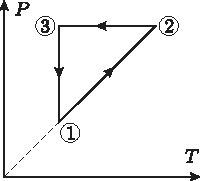
\includegraphics[width=0.4\linewidth]{2006-v2g-02-yl}
\end{center}
\fi


\ifHint
$P$-$V$ teljestikus avaldub gaasi tehtud töö tsükli aluse pindalana. Alternatiivselt võib iga tsükli etapil tehtud töö leidmiseks rakendada termodünaamika esimest seadust.
\fi


\ifSolution
Antud joonise saab teisendeda telgedega $P$ ja $V$ graafikuks, kus iga tsükli osa töö on arvuliselt võrdne antud graafiku osa alla jääva pindalaga (sest tehtud töö on $P\Delta V$). Ideaalse gaasi töö protsessi osal $1 \rightarrow 2$: $A_{1\rightarrow 2} = 0$, protsessi osal $2 \rightarrow 3$: $A_{2\rightarrow 3} < 0$ ning protsessi osal $3 \rightarrow 1$: $A_{3\rightarrow 1} > 0$, kuid $|A_2\rightarrow 3| > |A_3\rightarrow 1|$, seega $A_{1\rightarrow 2\rightarrow 3} < 0$, ehk gaasi tehtud töö on negatiivne.

\begin{center}
	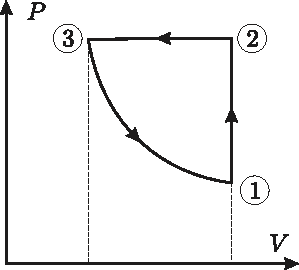
\includegraphics[width=0.4\linewidth]{2006-v2g-02-lah}
\end{center}
\fi
}